%%%%%%%%%%%%%%%%%%%%%%%%%%%%%%%%%%%%%%%%%%%%%%%%%%%%%%%%%%%%%%%%%%%%%
%
<<<<<<< HEAD
%  TEMPLATE LATEX — RELATÓRIO ACADÉMICO (ISEL)
=======
%  TEMPLATE LATEX — RELATÓRIO (ISEL)
>>>>>>> 2111bd995045ba7aacbb55b96df26ee9bcfc15e0
%  ============================================
%  Versão  : 1.0
%
%  INSTRUÇÕES RÁPIDAS
%  ------------------
%  1. Preenche as variáveis em "DADOS DO RELATÓRIO" (logo abaixo).
%  2. Substitui os textos "Lorem ipsum" pelo teu conteúdo.
%  3. Coloca as tuas imagens na pasta /images e atualiza os caminhos
%     em cada \includegraphics{}.
%  4. Compila com pdfLaTeX (duas vezes para o índice ficar correto).
%
%  ESTRUTURA DO FICHEIRO
%  ---------------------
%  [A] Pacotes e configurações globais
%  [B] Cabeçalho e rodapé (fancyhdr)
%  [C] Página de título
%  [D] Índice
%  [E] Corpo do relatório
%  [F] Referências
%  [G] Anexos
%
%  SNIPPETS ÚTEIS (no final do ficheiro)
%  → Figura, Tabela, Lista, Equação
%
%%%%%%%%%%%%%%%%%%%%%%%%%%%%%%%%%%%%%%%%%%%%%%%%%%%%%%%%%%%%%%%%%%%%%


% ===================================================================
% [0]  DADOS DO RELATÓRIO — preenche aqui
% ===================================================================
\newcommand{\relCadeira}{Nome da Cadeira}
\newcommand{\relAnoLetivo}{20XX / 20XX Verão/Inverno}
\newcommand{\relTitulo}{Título do Relatório}
\newcommand{\relSubtitulo}{Subtítulo (opcional)}
<<<<<<< HEAD
\newcommand{\relLicenciatura}{Licenciatura em Engenharia Informática e de Computadores}
=======
\newcommand{\relLicenciatura}{Licenciatura em XXXXX}
>>>>>>> 2111bd995045ba7aacbb55b96df26ee9bcfc15e0
\newcommand{\relAlunoA}{Aluno n.º XXXXX Nome Completo}
\newcommand{\relAlunoB}{Aluno n.º XXXXX Nome Completo}
\newcommand{\relDocente}{Nome do Docente}


% ===================================================================
% [A]  PACOTES E CONFIGURAÇÕES GLOBAIS
% ===================================================================
\documentclass[12pt]{article}

% --- Idioma e codificação ---
\usepackage[portuguese]{babel}
\usepackage[utf8]{inputenc}
\usepackage[T1]{fontenc}

% --- Página ---
\usepackage{geometry}
\geometry{
    a4paper,
    top=35mm,
    bottom=25mm,
    left=20mm,
    right=20mm,
    headsep=20pt
}

% --- Gráficos e figuras ---
\usepackage{graphicx}
\usepackage{subcaption}
\usepackage{wrapfig}
\usepackage[font=small, labelfont=bf]{caption}
\usepackage{float}

% --- Tipografia ---
\usepackage{setspace}
\onehalfspacing
\usepackage{microtype}

% --- Matemática ---
\usepackage{amsmath}
\usepackage{amsfonts}
\usepackage{amssymb}

% --- Tabelas ---
\usepackage{booktabs}
\usepackage{array}

% --- Listas ---
\usepackage{enumitem}

% --- Cores ---
\usepackage{xcolor}

% --- Hiperligações ---
\usepackage{hyperref}
\hypersetup{
    colorlinks = true,
    linkcolor  = black,
    urlcolor   = blue,
    citecolor  = black
}

% --- URL ---
\usepackage{url}

% --- Cabeçalho e rodapé ---
\usepackage{fancyhdr}

% --- Numeração de secções com ponto (ex: "1.") ---
\usepackage{titlesec}
\titlelabel{\thetitle.\quad}


% ===================================================================
% [B]  CABEÇALHO E RODAPÉ
% ===================================================================
\pagestyle{fancy}
\fancyhf{} % limpa tudo antes de definir

\setlength{\headheight}{45pt}

<<<<<<< HEAD
% Cabeçalho: logo à esquerda, texto à direita
=======
% Cabeçalho
>>>>>>> 2111bd995045ba7aacbb55b96df26ee9bcfc15e0
\fancyhead[C]{%
    \makebox[\textwidth]{%
        
\includegraphics[height=1.2cm]{images/logo-isel.png}%
        \hfill%
        \begin{tabular}[b]{r}
            \relCadeira \\
            \relAnoLetivo \\
            \relTitulo\ (\textit{\relSubtitulo})
        \end{tabular}%
    }%
}

<<<<<<< HEAD
% Linha vermelha sob o cabeçalho
=======
% Linha vermelha sob o cabeçalhoS
>>>>>>> 2111bd995045ba7aacbb55b96df26ee9bcfc15e0
\renewcommand{\headrulewidth}{0pt} % desativa a linha padrão do fancyhdr
\renewcommand{\headrule}{%
    \vspace{-4pt}%
    {\color{red!60!black}\makebox[\textwidth]{\rule{\textwidth}{1.5pt}}}%
}

% Rodapé: número de página centrado
\fancyfoot[C]{\thepage}


% ===================================================================
% [C]  INÍCIO DO DOCUMENTO
% ===================================================================
\begin{document}

% -------------------------------------------------------------------
% Página de título
% -------------------------------------------------------------------
\begin{titlepage}
    \thispagestyle{empty}
    \centering

    
\includegraphics[scale=0.8]{images/iselnewlogo.png}\\[1.5cm]

<<<<<<< HEAD
    \relLicenciatura\\[2cm]
=======
    \large \relLicenciatura\\[2cm]
>>>>>>> 2111bd995045ba7aacbb55b96df26ee9bcfc15e0

    {\LARGE \textbf{\relTitulo}}\\[0.4em]
    {\Large \relSubtitulo}\\[2cm]

    \begin{flushleft}
        Trabalho realizado por:
        \begin{itemize}[label={}]
            \item \relAlunoA
            \item \relAlunoB
        \end{itemize}

        \vspace{0.5cm}
        Docente: \relDocente
    \end{flushleft}

    \vfill

    {\relCadeira}\\[0.3em]
    {\relAnoLetivo}

\end{titlepage}


% ===================================================================
% [D]  ÍNDICE  (numeração romana)
% ===================================================================
\setcounter{page}{1}
\pagenumbering{roman}
\thispagestyle{empty}
\addcontentsline{toc}{section}{\protect\numberline{}Índice}
\tableofcontents
\newpage


% ===================================================================
% [E]  CORPO DO RELATÓRIO  (numeração árabe)
% ===================================================================
\pagenumbering{arabic}
\setcounter{page}{1}

% -------------------------------------------------------------------
\section{Secção 1 — Título}
% -------------------------------------------------------------------

\par Primeiro parágrafo:
Lorem ipsum dolor sit amet, consectetuer adipiscing elit. Aenean commodo ligula eget dolor.
Aenean massa. Cum sociis natoque penatibus et magnis dis parturient montes, nascetur
ridiculus mus. Donec quam felis, ultricies nec, pellentesque eu, pretium quis, sem.
Nulla consequat massa quis enim. Donec pede justo, fringilla vel, aliquet nec, vulputate
eget, arcu.

\begin{figure}[h]
    \centering
    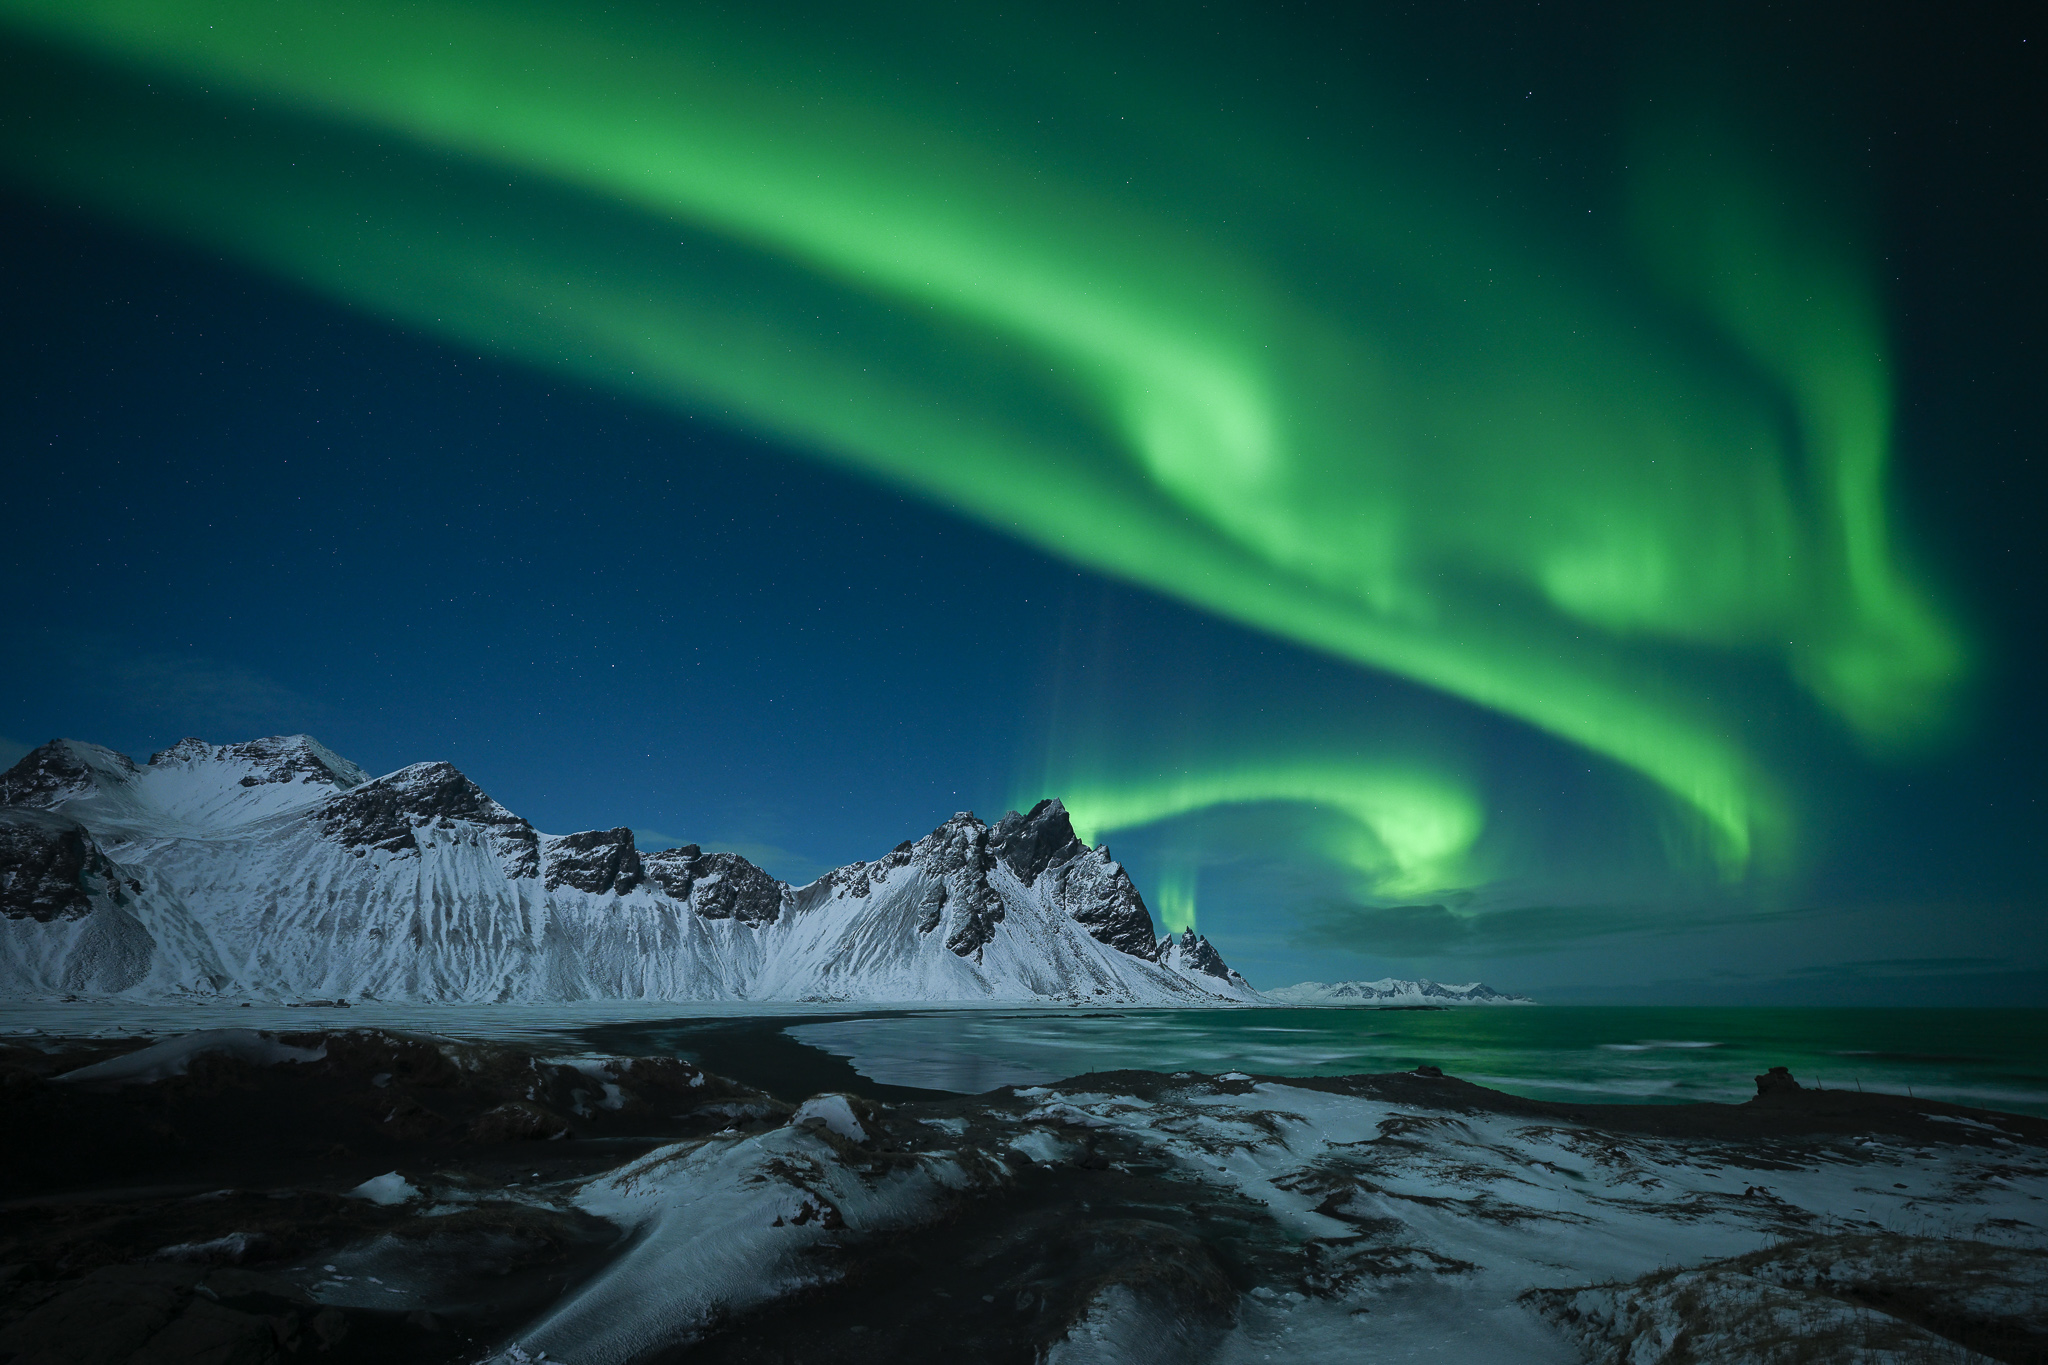
\includegraphics[width=0.75\textwidth]{images/sampleimage.jpg}
    \caption{Descrição da imagem.}
    \label{fig:imagem1}
\end{figure}

\clearpage

% -------------------------------------------------------------------
\section{Secção 2 — Título}
% -------------------------------------------------------------------

% - - - - - - - - - - - - - - - - - - - - - - - - - - - - - - - - -
\subsection{Subsecção 2.1 — Título}
% - - - - - - - - - - - - - - - - - - - - - - - - - - - - - - - - -

\begin{center}
    \texttt{Texto centrado — exemplo de assinatura de função}
\end{center}

Lorem ipsum dolor sit amet, consectetuer adipiscing elit. Aenean commodo ligula eget dolor.
Aenean massa. Cum sociis natoque penatibus et magnis dis parturient montes, nascetur
ridiculus mus. Donec quam felis, ultricies nec, pellentesque eu, pretium quis, sem.

% - - - - - - - - - - - - - - - - - - - - - - - - - - - - - - - - -
\subsection{Subsecção 2.2 — Título}
% - - - - - - - - - - - - - - - - - - - - - - - - - - - - - - - - -

\begin{center}
    \texttt{Texto centrado — Lorem ipsum dolor sit amet.}
\end{center}

Lorem ipsum dolor sit amet, consectetuer adipiscing elit. Aenean commodo ligula eget dolor.
Aenean massa. Cum sociis natoque penatibus et magnis dis parturient montes.

% - - - - - - - - - - - - - - - - - - - - - - - - - - - - - - - - -
\subsection{Subsecção 2.3 — Título}
% - - - - - - - - - - - - - - - - - - - - - - - - - - - - - - - - -

Lorem ipsum dolor sit amet, consectetuer adipiscing elit. Aenean commodo ligula eget dolor.

\begin{figure}[h]
    \centering
    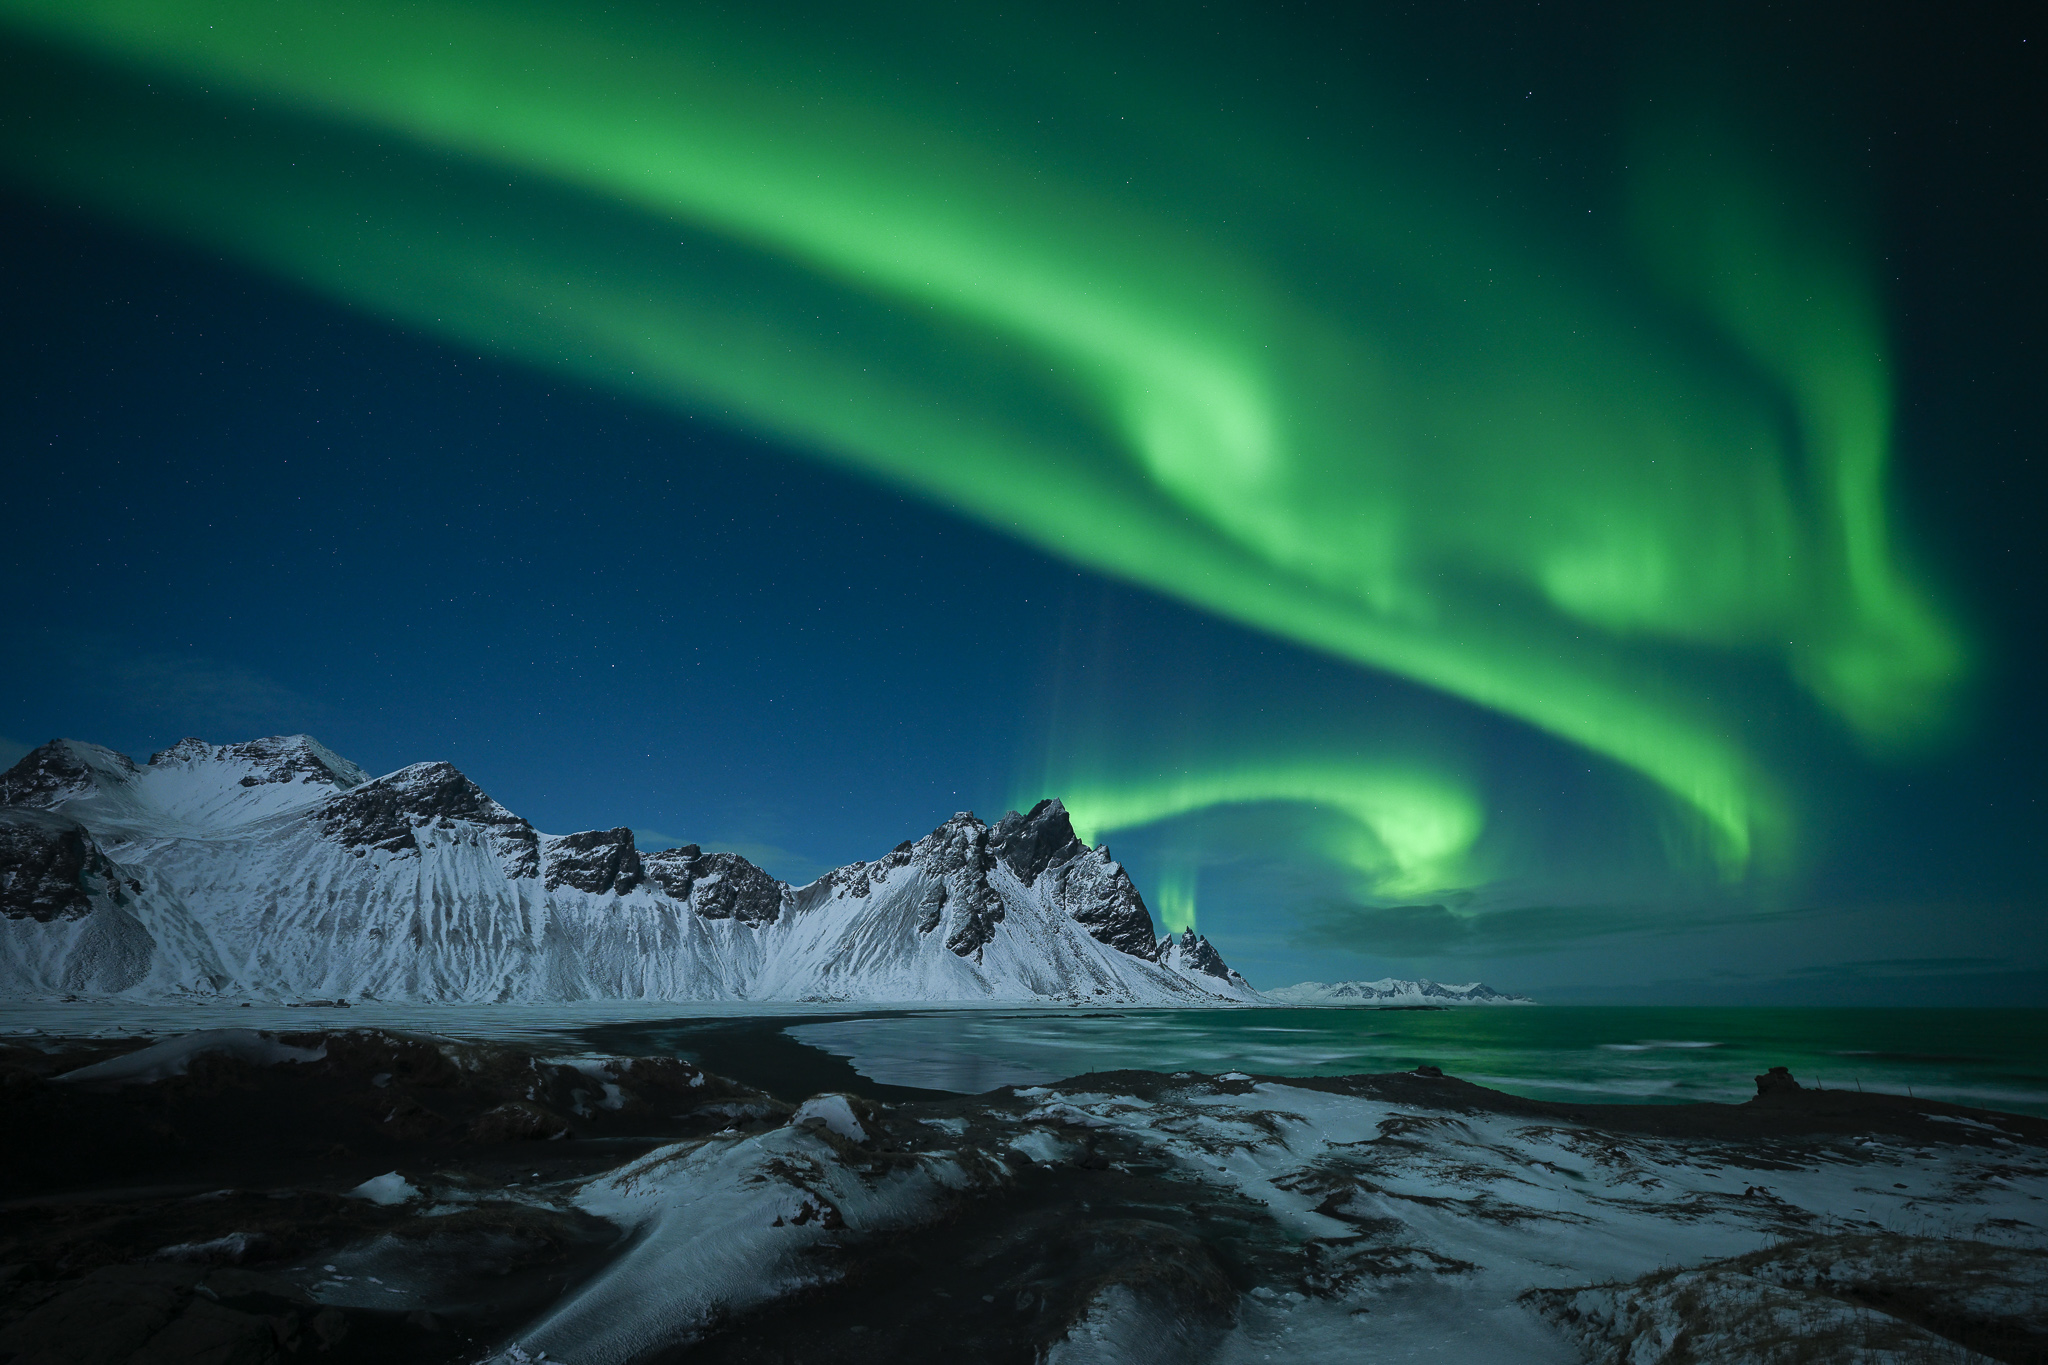
\includegraphics[width=0.85\textwidth]{images/sampleimage.jpg}
    \caption{Descrição da imagem.}
    \label{fig:imagem2}
\end{figure}

% -------------------------------------------------------------------
\section{Secção 3 — Título}
% -------------------------------------------------------------------

Lorem ipsum dolor sit amet, consectetuer adipiscing elit. Aenean commodo ligula eget dolor.
Aenean massa. Cum sociis natoque penatibus et magnis dis parturient montes, nascetur
ridiculus mus. Donec quam felis, ultricies nec, pellentesque eu, pretium quis, sem.

\begin{figure}[h]
    \centering
    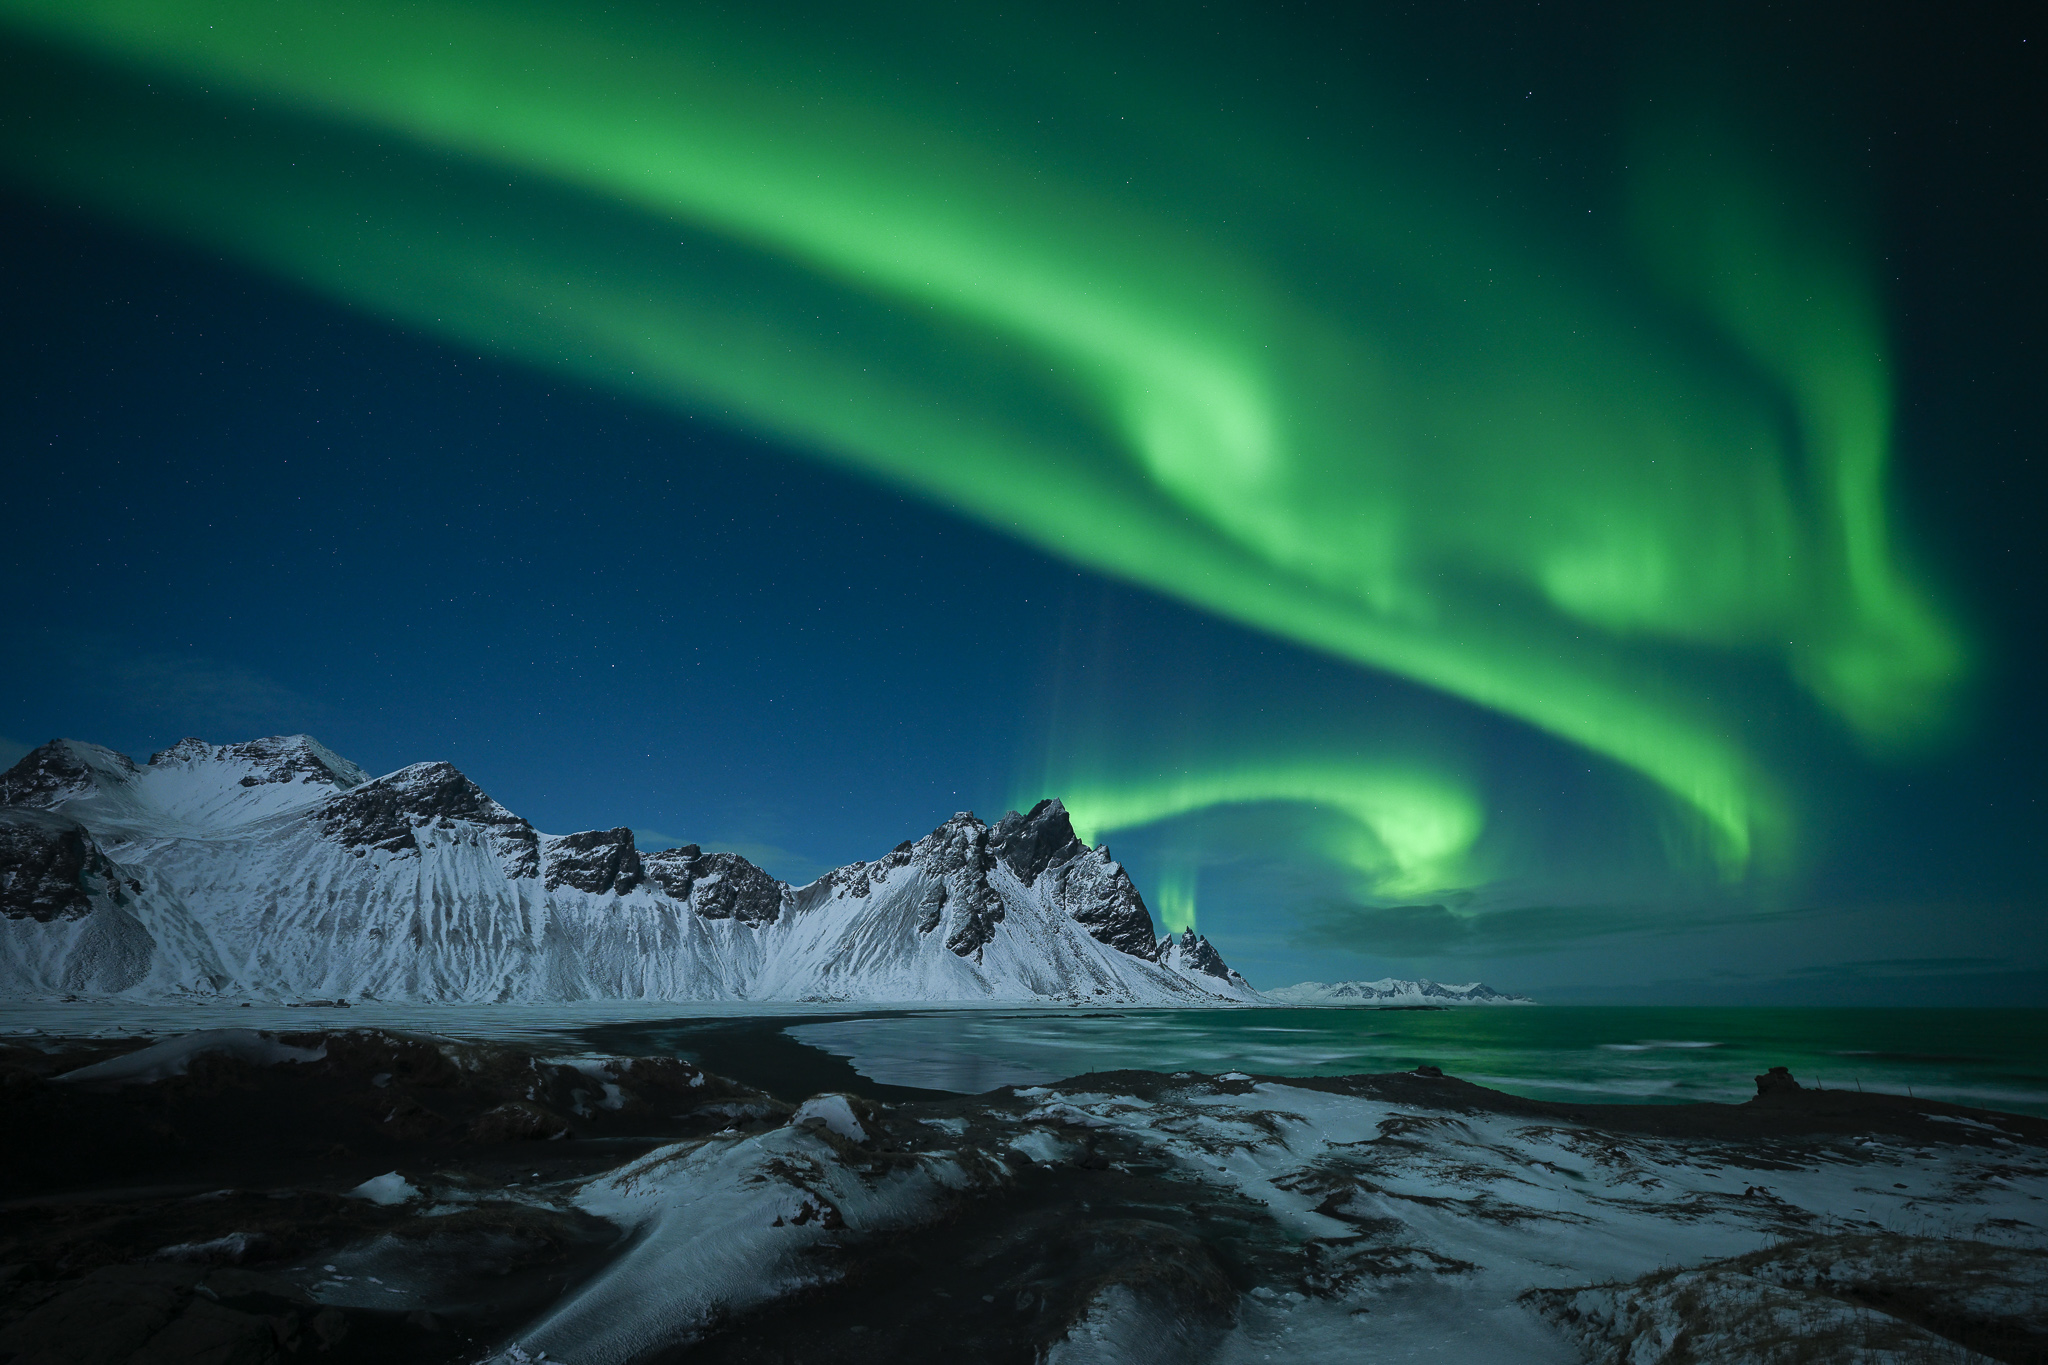
\includegraphics[width=0.95\textwidth]{images/sampleimage.jpg}
    \caption{Descrição da imagem.}
    \label{fig:imagem3}
\end{figure}

% -------------------------------------------------------------------
\section{Secção 4 — Título}
% -------------------------------------------------------------------

% - - - - - - - - - - - - - - - - - - - - - - - - - - - - - - - - -
\subsection{Subsecção 4.1 — Título}
% - - - - - - - - - - - - - - - - - - - - - - - - - - - - - - - - -

Lorem ipsum dolor sit amet, consectetuer adipiscing elit. Aenean commodo ligula eget dolor.

% - - - - - - - - - - - - - - - - - - - - - - - - - - - - - - - - -
\subsection{Subsecção 4.2 — Título}
% - - - - - - - - - - - - - - - - - - - - - - - - - - - - - - - - -

Lorem ipsum dolor sit amet, consectetuer adipiscing elit. Aenean commodo ligula eget dolor.

\subsubsection{Subsubsecção 4.2.1 — Título}
\label{sec:sub421}

\begin{itemize}
    \item Lorem ipsum dolor sit amet, consectetuer adipiscing elit.
    \item Lorem ipsum dolor sit amet, consectetuer adipiscing elit.
\end{itemize}

\subsubsection{Subsubsecção 4.2.2 — Título}
\label{sec:sub422}

\begin{itemize}
    \item Lorem ipsum dolor sit amet, consectetuer adipiscing elit.
    \item Lorem ipsum dolor sit amet, consectetuer adipiscing elit.
    \item Lorem ipsum dolor sit amet, consectetuer adipiscing elit.
\end{itemize}

\begin{figure}[h]
    \centering
    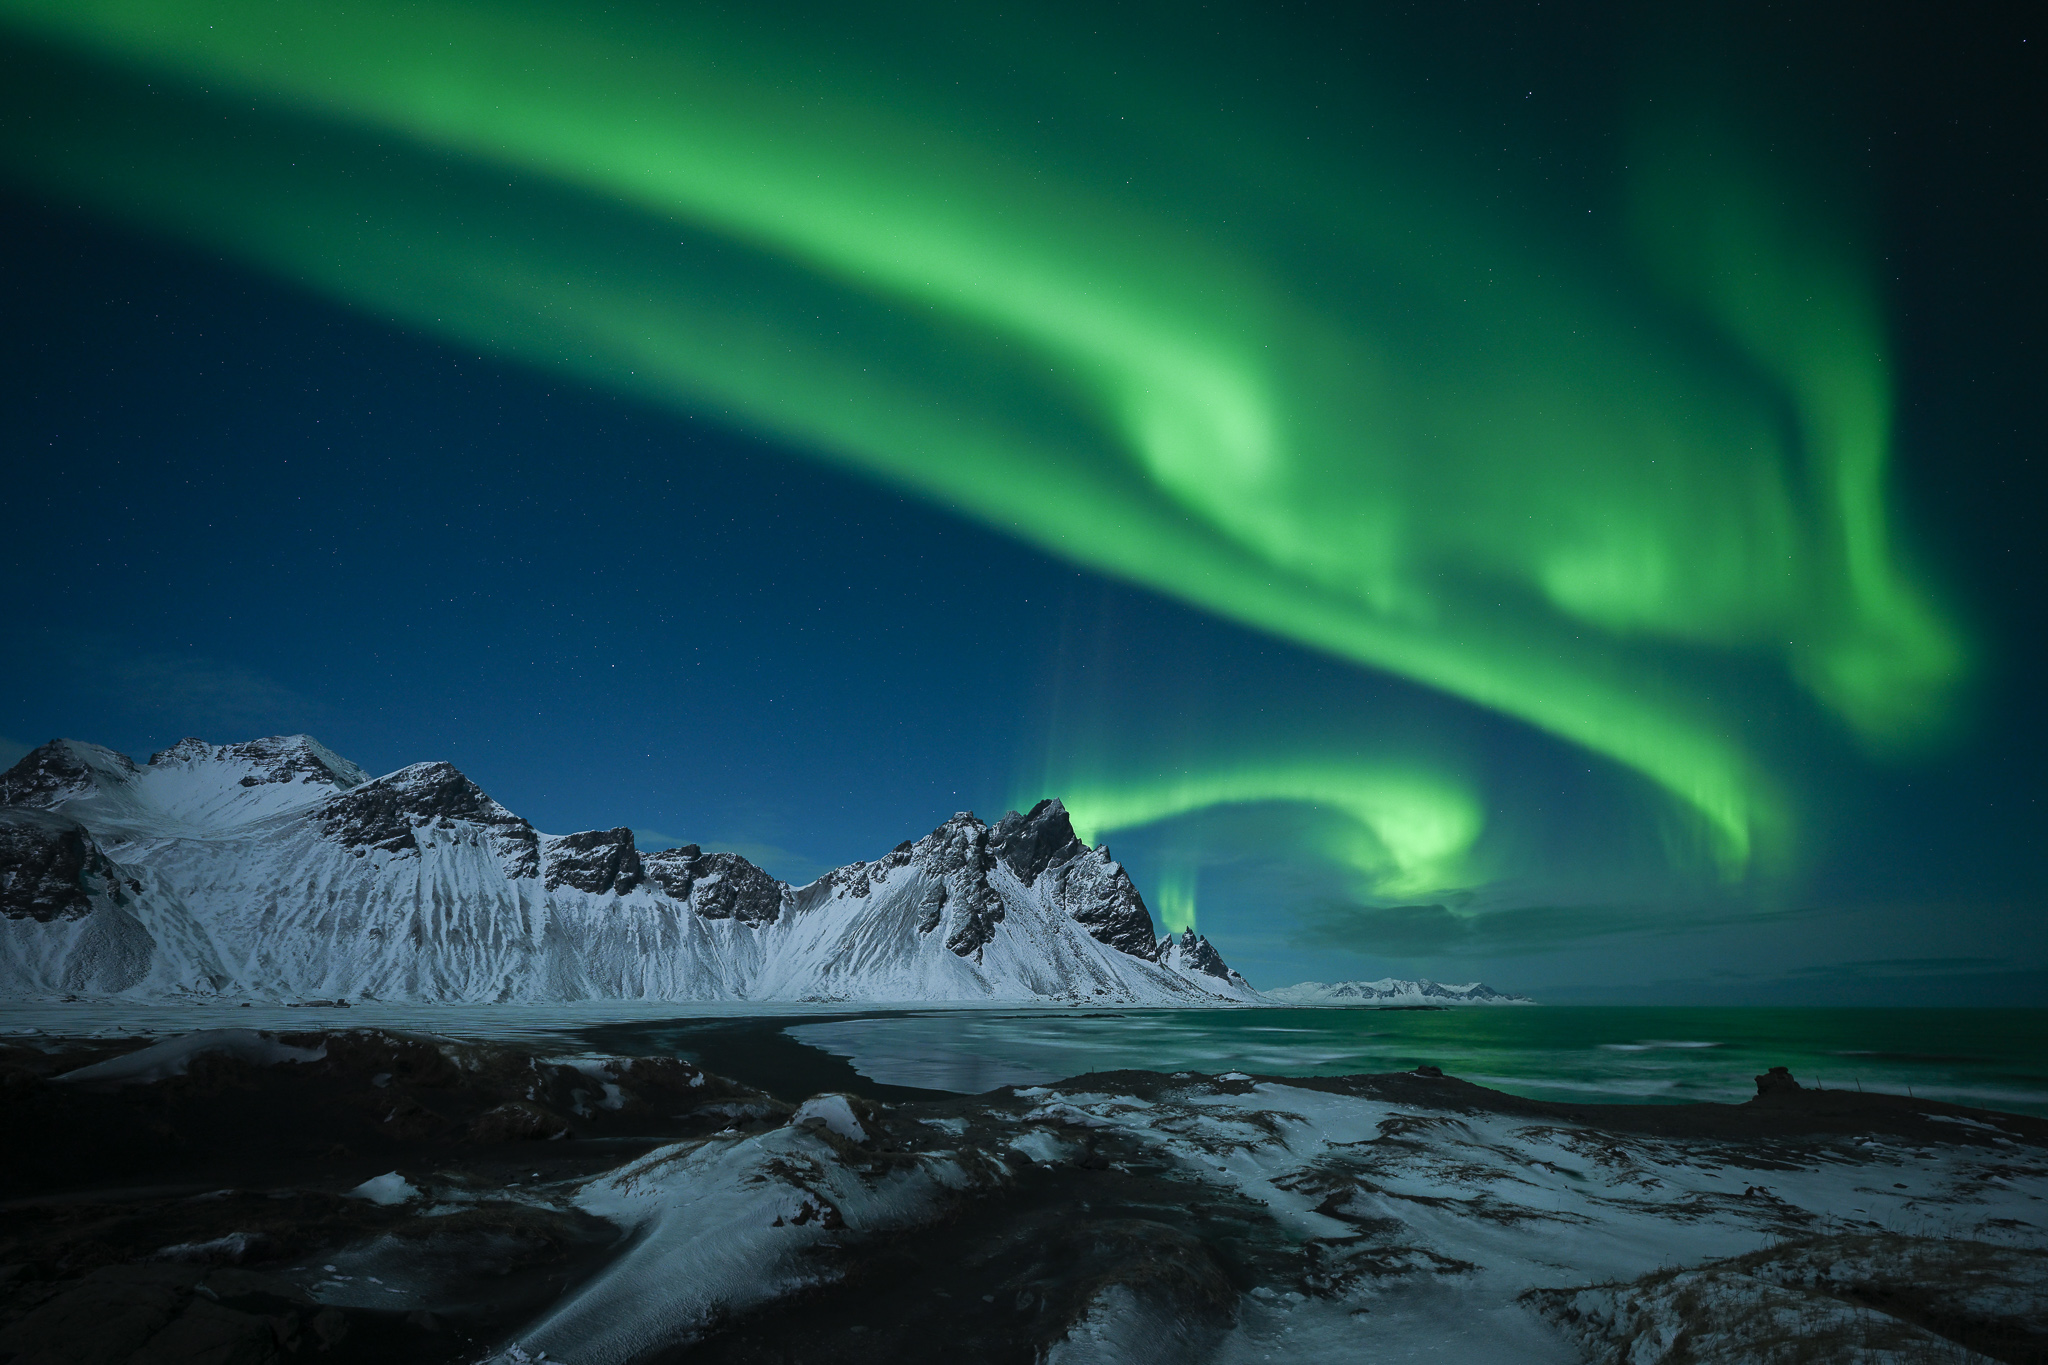
\includegraphics[width=0.65\textwidth]{images/sampleimage.jpg}
    \caption{Descrição da imagem.}
    \label{fig:imagem4}
\end{figure}

Lorem ipsum dolor sit amet, consectetuer adipiscing elit. Aenean commodo ligula eget dolor.

\begin{figure}[h]
    \centering
    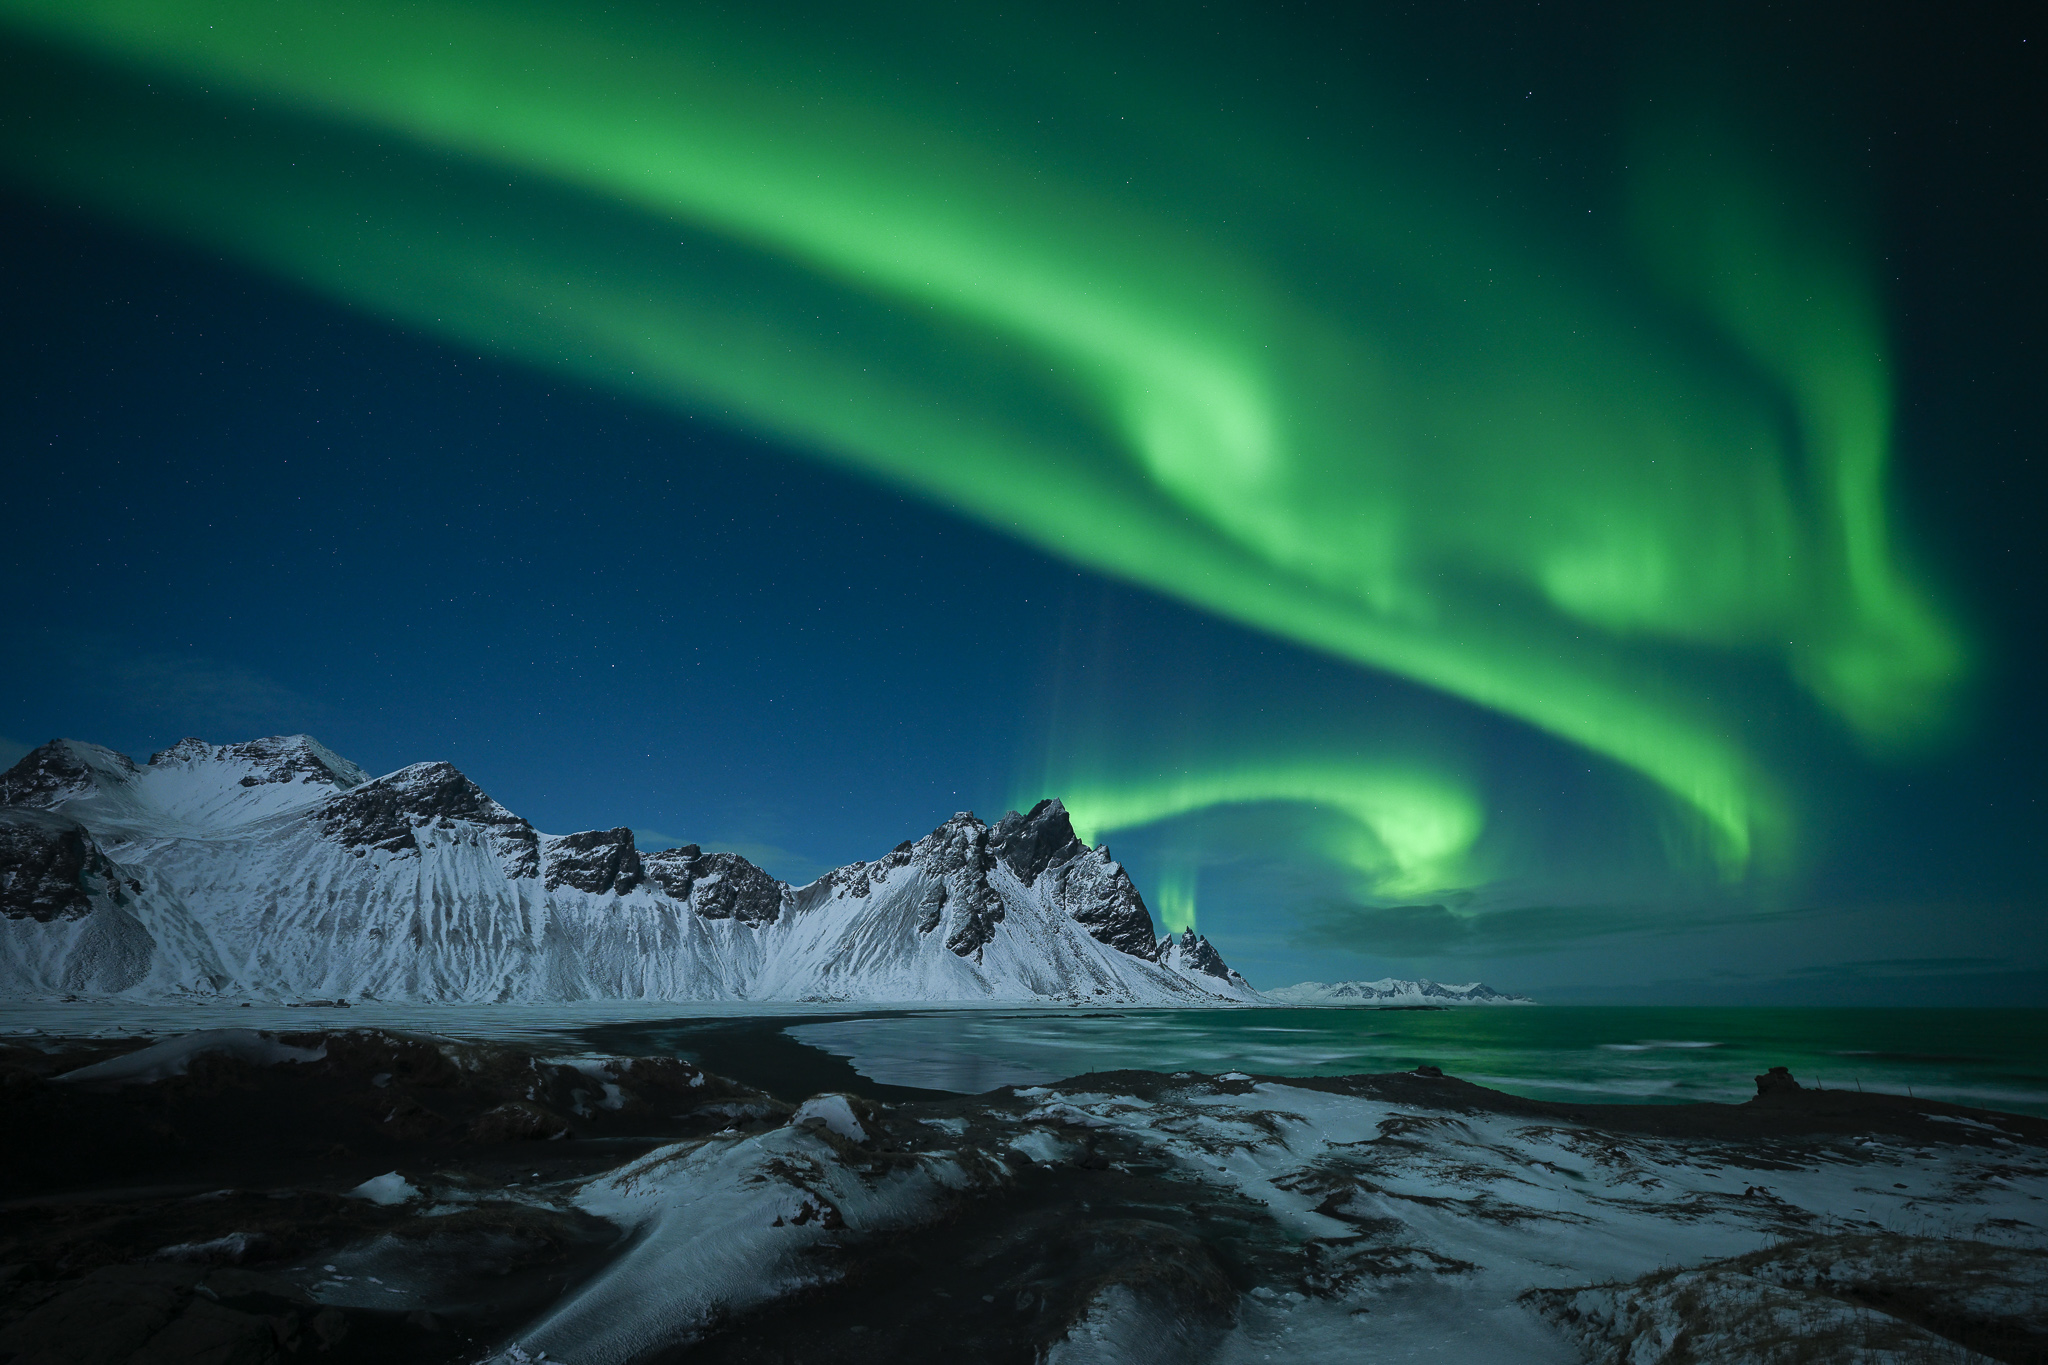
\includegraphics[width=0.95\textwidth]{images/sampleimage.jpg}
    \caption{Descrição da imagem.}
    \label{fig:imagem5}
\end{figure}

% - - - - - - - - - - - - - - - - - - - - - - - - - - - - - - - - -
\subsection{Subsecção 4.3 — Título}
\label{sec:algoritmos}
% - - - - - - - - - - - - - - - - - - - - - - - - - - - - - - - - -

\subsubsection*{Implementação 1}

\begin{itemize}
    \item Lorem ipsum dolor sit amet, consectetuer adipiscing elit.
    \item Lorem ipsum dolor sit amet, consectetuer adipiscing elit.
    \item Lorem ipsum dolor sit amet, consectetuer adipiscing elit.
\end{itemize}

\subsubsection*{Implementação 2}

\begin{itemize}
    \item Lorem ipsum dolor sit amet, consectetuer adipiscing elit.
    \item Lorem ipsum dolor sit amet, consectetuer adipiscing elit.
    \item Lorem ipsum dolor sit amet, consectetuer adipiscing elit.
\end{itemize}

\textbf{Nota:} Lorem ipsum dolor sit amet, consectetuer adipiscing elit.

\subsubsection*{Análise detalhada}

Lorem ipsum dolor sit amet, consectetuer adipiscing elit. Aenean commodo ligula eget dolor.
Aenean massa. Cum sociis natoque penatibus et magnis dis parturient montes.

\begin{figure}[h]
    \centering
    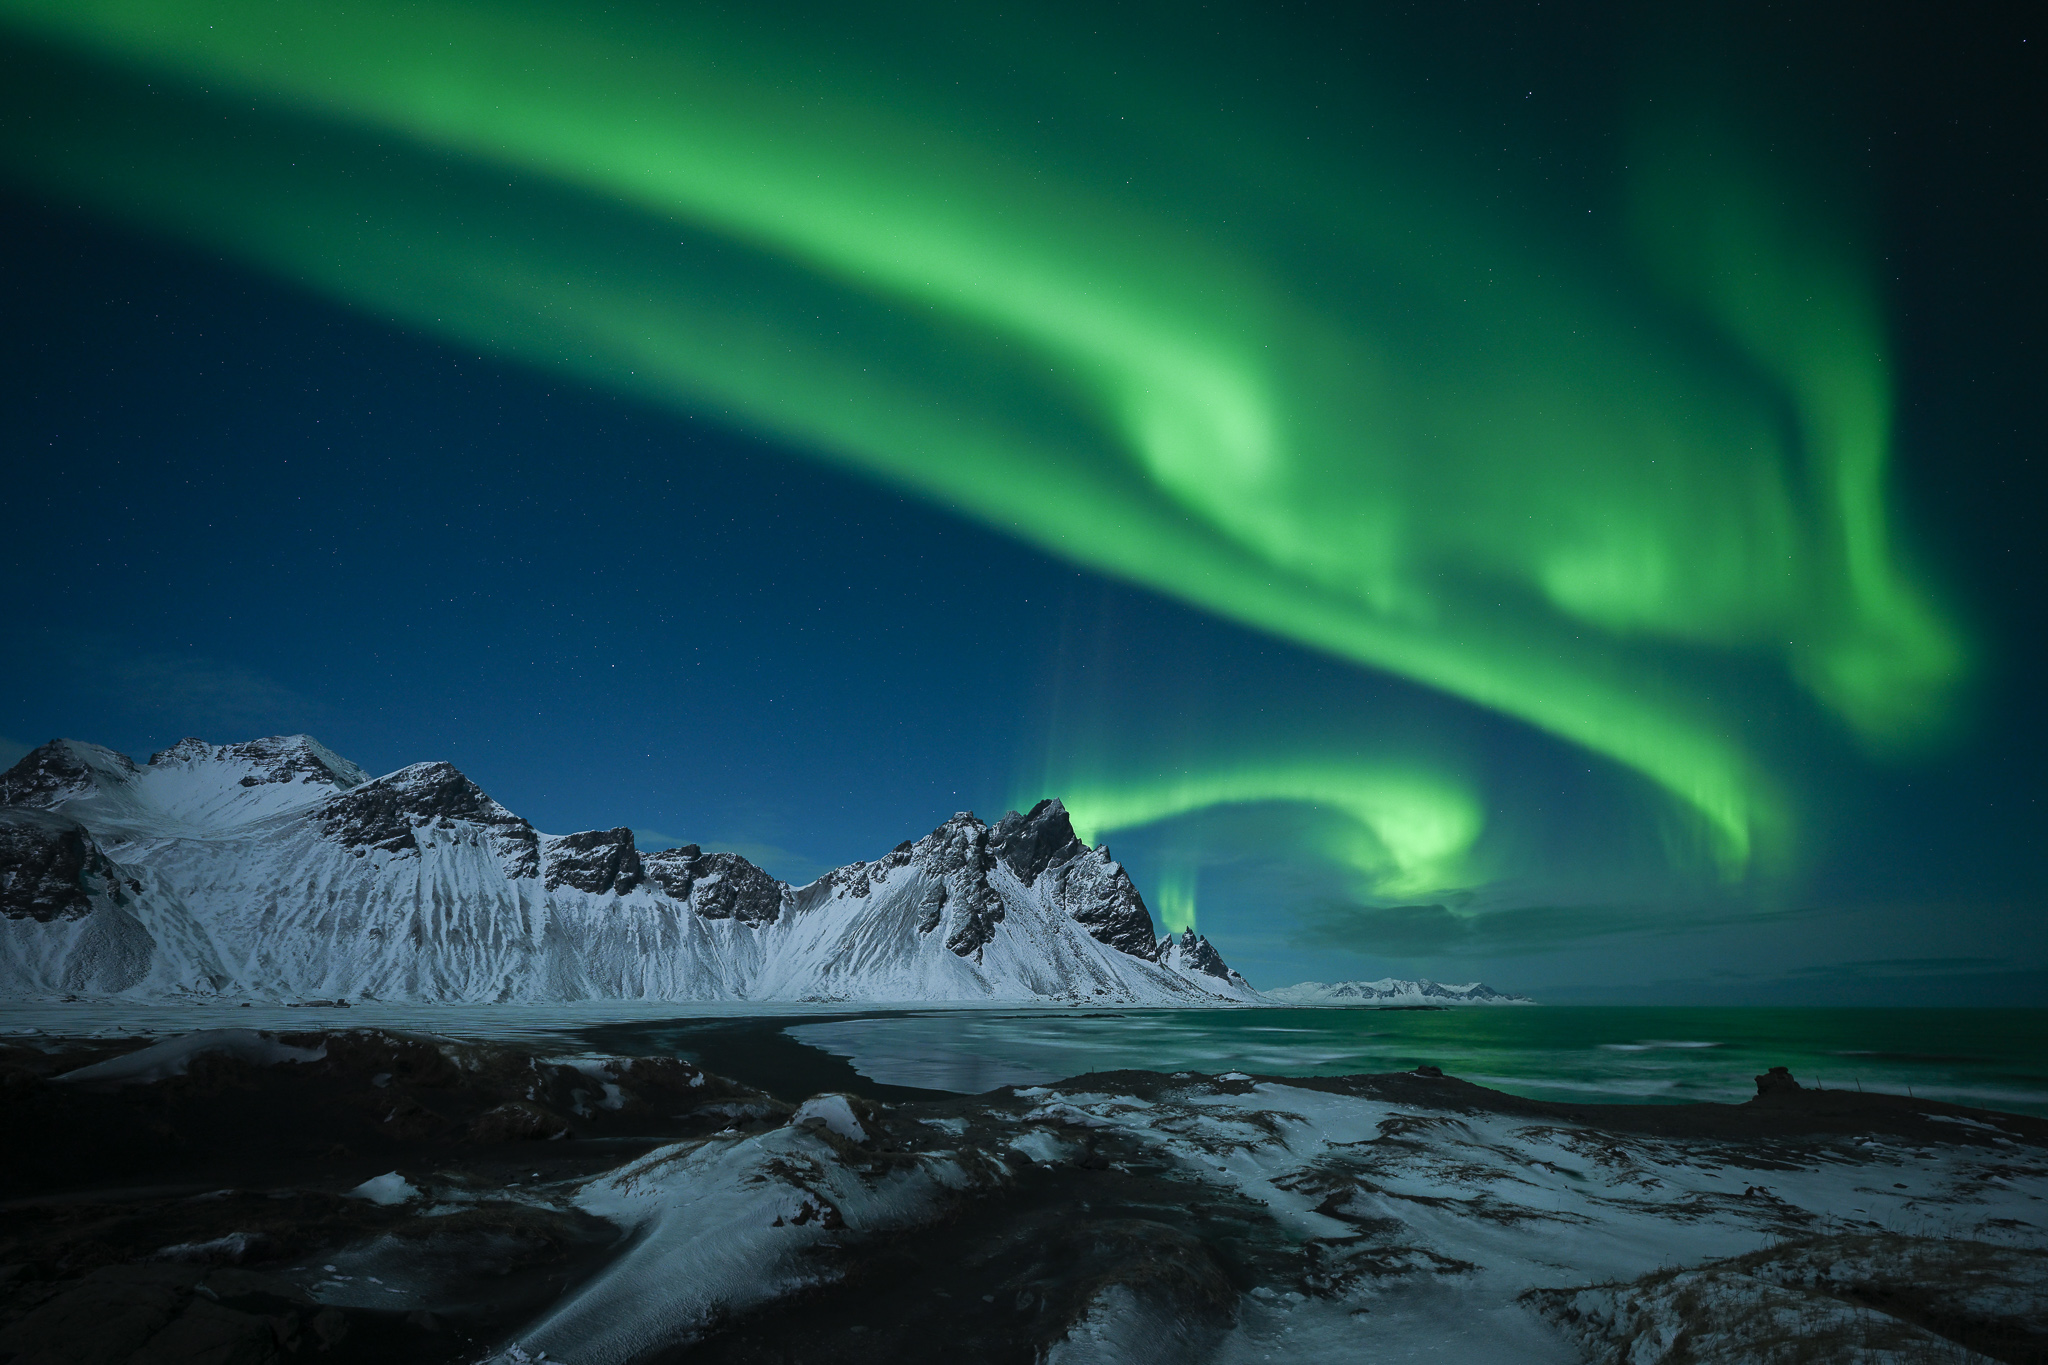
\includegraphics[width=0.4\textwidth]{images/sampleimage.jpg}
    \caption{Descrição da imagem.}
    \label{fig:imagem6}
\end{figure}

% - - - - - - - - - - - - - - - - - - - - - - - - - - - - - - - - -
\subsection{Subsecção 4.4 — Avaliação Experimental}
\label{sec:experimental}
% - - - - - - - - - - - - - - - - - - - - - - - - - - - - - - - - -

Lorem ipsum dolor sit amet, consectetuer adipiscing elit. Aenean commodo ligula eget dolor.

\begin{figure}[h]
    \centering
    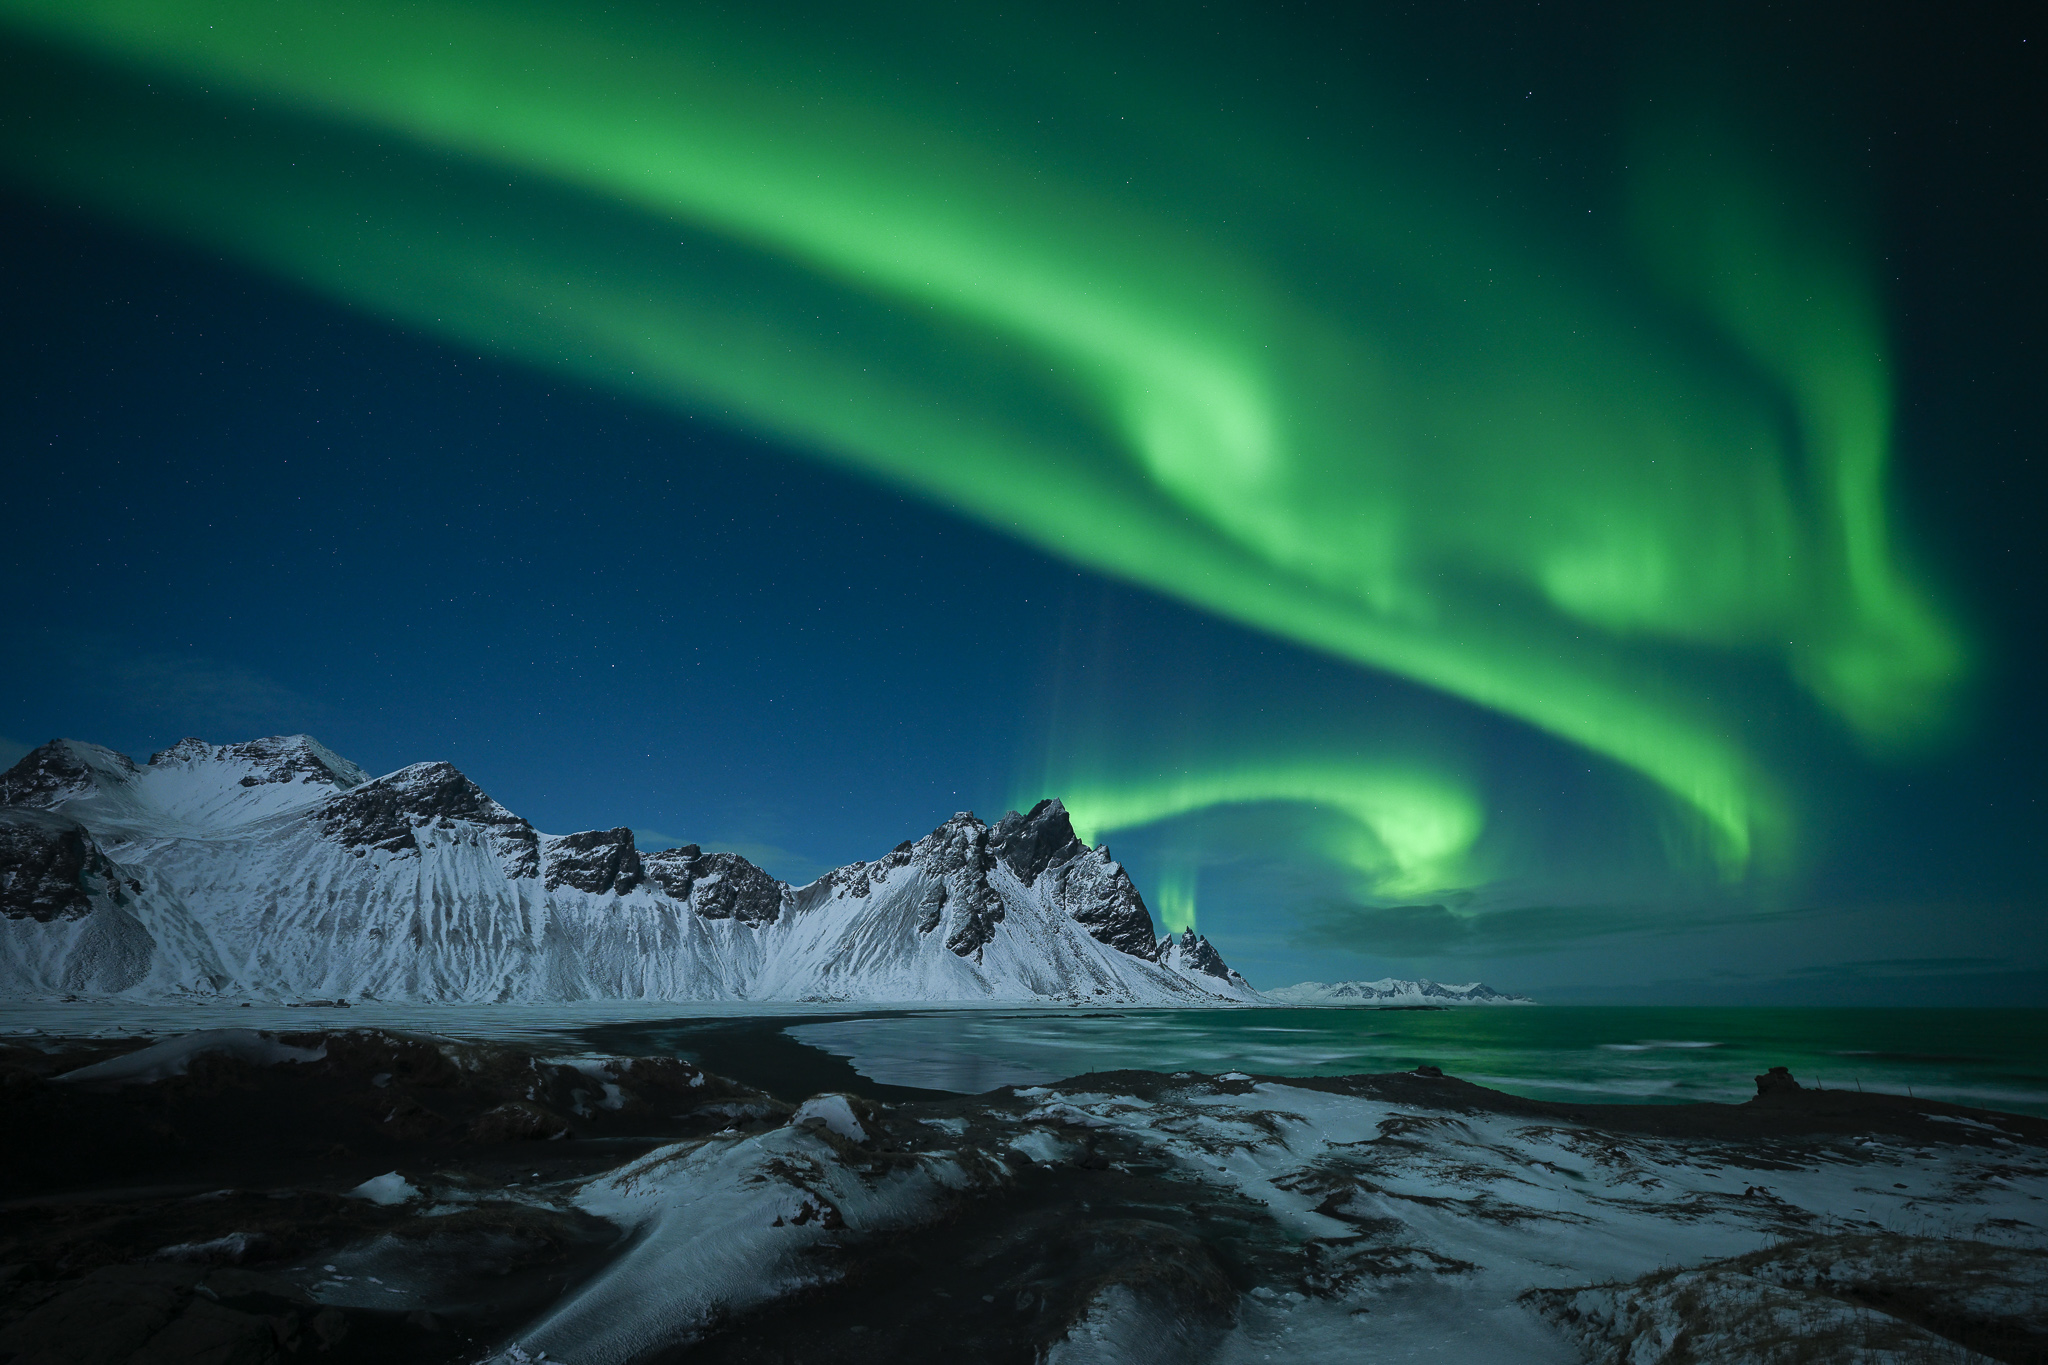
\includegraphics[width=0.9\textwidth]{images/sampleimage.jpg}
    \caption{Tabela de resultados experimentais.}
    \label{fig:tabela}
\end{figure}

\begin{figure}[h]
    \centering
    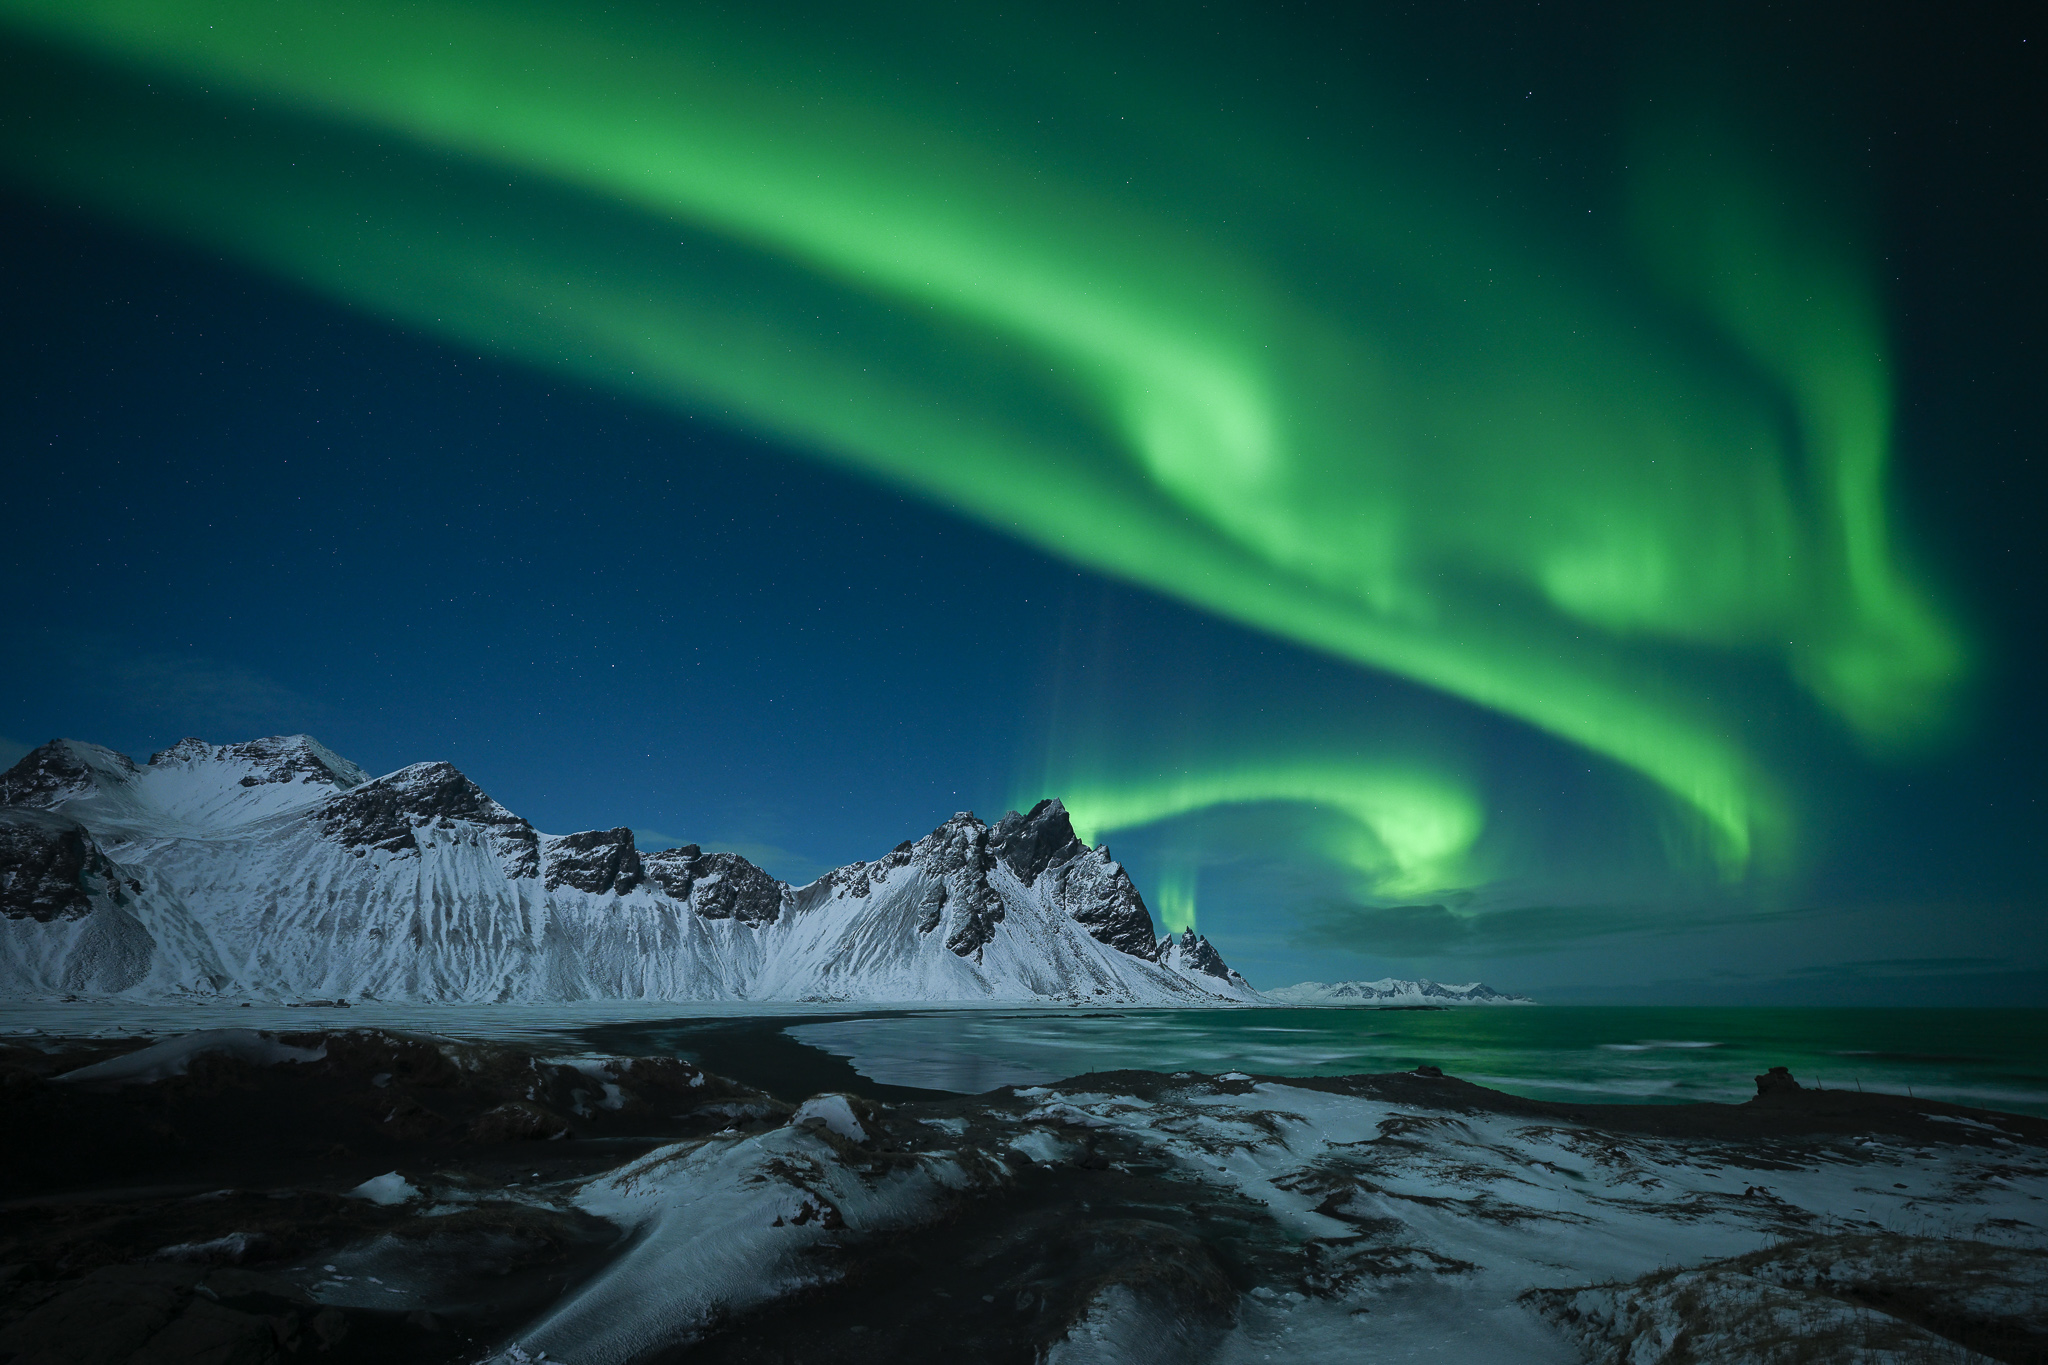
\includegraphics[width=0.95\textwidth]{images/sampleimage.jpg}
    \caption{Gráfico comparativo.}
    \label{fig:grafico}
\end{figure}

Lorem ipsum dolor sit amet, consectetuer adipiscing elit. Aenean commodo ligula eget dolor.

% - - - - - - - - - - - - - - - - - - - - - - - - - - - - - - - - -
\subsection{Subsecção 4.5 — Conclusões}
\label{sec:conclusoes}
% - - - - - - - - - - - - - - - - - - - - - - - - - - - - - - - - -

Lorem ipsum dolor sit amet, consectetuer adipiscing elit. Aenean commodo ligula eget dolor.
Aenean massa. Cum sociis natoque penatibus et magnis dis parturient montes, nascetur
ridiculus mus.


% ===================================================================
% [F]  REFERÊNCIAS
% ===================================================================
\newpage
\section*{Referências}
\addcontentsline{toc}{section}{\protect\numberline{}Referências}

\begin{thebibliography}{9}

\bibitem{moodle}
Nome do Autor,
\textit{Título do Recurso}.
Disponível em: \url{https://XXXX.moodle.isel.pt}.

\bibitem{clrs}
2ª Referencia

\end{thebibliography}


% ===================================================================
% [G]  ANEXOS
% ===================================================================
\appendix
\clearpage
\section{Anexos}

<<<<<<< HEAD
=======
\large Neste bloco podes colocar o que tu quiseres sendo código, imagens de avaliações experimentais, gráficos, dados de X, etc...

>>>>>>> 2111bd995045ba7aacbb55b96df26ee9bcfc15e0
% Insere aqui o conteúdo dos anexos, por exemplo código-fonte:
%
% \subsection{Ficheiro Main.kt}
% \inputminted[breaklines]{kotlin}{src/Main.kt}
<<<<<<< HEAD
=======
% Na inputminted[breaklines]{kotlin}{src/Main.kt} a única alteração a ser %feita deve ser no bloco {src/Main.kt} no qual devas criar uma pasta de nome %á tua escolha, preferencialmente de nome intuitivo ao anexo em questão. De %seguida, devos colocar os ficheiros .yy na pasta que criaste e alterar o {stc/Main.kt} com o nome da pasta e do ficheiro localizado na pasta. 
>>>>>>> 2111bd995045ba7aacbb55b96df26ee9bcfc15e0

\end{document}


%%%%%%%%%%%%%%%%%%%%%%%%%%%%%%%%%%%%%%%%%%%%%%%%%%%%%%%%%%%%%%%%%%%%%
%  SNIPPETS — copia e cola onde precisares
%%%%%%%%%%%%%%%%%%%%%%%%%%%%%%%%%%%%%%%%%%%%%%%%%%%%%%%%%%%%%%%%%%%%%
%
% -- FIGURA --------------------------------------------------------
%\begin{figure}[h]
%    \centering
%    \includegraphics[width=0.8\textwidth]{images/nome_ficheiro.png}
%    \caption{Descrição da figura.}
%    \label{fig:nome_unico}
%\end{figure}
%
% -- TABELA --------------------------------------------------------
%\begin{table}[h]
%    \centering
%    \begin{tabular}{|l|c|r|}
%        \hline
%        \textbf{Coluna A} & \textbf{Coluna B} & \textbf{Coluna C} \\ \hline
%        Valor 1           & Valor 2           & Valor 3           \\ \hline
%    \end{tabular}
%    \caption{Descrição da tabela.}
%    \label{tab:nome_unico}
%\end{table}
%
% -- LISTA COM PONTOS ----------------------------------------------
%\begin{itemize}
%    \item Primeiro item.
%    \item Segundo item.
%\end{itemize}
%
% -- LISTA NUMERADA ------------------------------------------------
%\begin{enumerate}
%    \item Primeiro item.
%    \item Segundo item.
%\end{enumerate}
%
% -- EQUAÇÃO -------------------------------------------------------
%\begin{equation}
%    E = mc^2
%    \label{eq:einstein}
%\end{equation}
%
% -- REFERÊNCIA A FIGURA/TABELA/EQUAÇÃO ----------------------------
% Ver Figura~\ref{fig:nome_unico}
% Ver Tabela~\ref{tab:nome_unico}
% Ver Equação~\eqref{eq:einstein}
%
%%%%%%%%%%%%%%%%%%%%%%%%%%%%%%%%%%%%%%%%%%%%%%%%%%%%%%%%%%%%%%%%%%%%%